


\section{Map-Relative Output Decoding}
\label{sec:supp_output}
Our output decoding can be divided into three steps: predicting the final goal
of an actor based on node embeddings, propose an initial trajectory based on the
goal and the initial pose, and refine the trajectory proposal with a learnable
header. As the first step is straight-forward, we now explain how we perform the
second and third steps in details.

\subsection{Trajectory Proposal}
Given a predicted final pose $\left(x^T, y^T, dx^T, dy^T\right)$ and initial
pose $\left(x^0,
y^0, dx^0, dy^0\right)$ of an actor, where $(x, y)$ is the 2D location and $(dx, dy)$
is the tangent vector, we fit a Bezier quadratic curve satisfying these boundary
conditions, \ie, zero-th and first order derivative values. Specifically, the curve can be parameterized by 
\begin{align}
  \nonumber
  x(s) &= a_0 s^2 + a_1 s + a_2,
  \\
  \nonumber
  y(s) &= b_0 s^2 + b_1 s + b_2,
  \\
  \nonumber
  s.t. \quad x(0) &= x^0, \quad x(1) = x^T, \quad \frac{x'(0)}{x'(1)} = \frac{dx^0}{dx^T},
  \\
  \nonumber
  y(0) &= y^0, \quad y(1) = y^T,  \quad \frac{y'(0)}{y'(1)} =
  \frac{dy^0}{dy^T}.
\end{align}
Here, $s$ is the normalized distance.
As a result, each predicted goal uniquely defines a 2D curve.

Next, we unroll a velocity profile along this curve to get 2D waypoint proposals
at every future timestamp. Assuming the actor is moving with a constant
acceleration within the prediction horizon, we can compute the acceleration
based on the initial velocity $v$ and the traveled distance $s$ (from
$(x^0, y^0)$ to $(x^T, y^T)$ along the Bezier curve) using
$$
a = \frac{2\times(s - vT)}{T^2}.
$$
Therefore, the future position of the actor at any timestamp $t$ can be
evaluated by querying the position along the curve at $s(t) = vt +
\frac{1}{2}at^2$.

\subsection{Trajectory Refinement}
Simply using our trajectory proposals for motion forecasting
will not be very accurate, as not all actors
move with constant accelerations and follow Bezier curves, yet the proposals
provide us good initial estimations which we can further refine. To do
so, for each trajectory proposal, we construct its features using a shortcut
layer on top our \ROI node embeddings. We then use a 2 layer MLP to decode a
pair of values $\left(s^t, d^t\right)$ for each future timestamp, representing
the actor position at time $t$ in the Frenet Coordinate System~\cite{frenet}.
The Cartesian coordinates $\left(x^t, y^t\right)$ can be mapped from
$\left(s^t, d^t\right)$ by first traversing along the Bezier curve distance
$s^t$ (\aka longitudinal), and then deviating perpendicularly from the curve
distance $d^t$ (\aka lateral). The sign of $d^t$ indicates the deviation is
either to-the-left or to-the-right.


\begin{table*}[t]
  \centering
  \begin{tabular}{ccc|ccccc}
  \specialrule{.2em}{.1em}{.1em}
  Sampling & Avg Length ($\ell_k$) & Reg & $\text{min}_1$ADE & $\text{min}_1$FDE & $\text{min}_6$ADE & $\text{min}_6$FDE & $\text{min}_6$MR\\
  \hline
  up 1x & 2.1 m& & 1.52 & 3.32 & 0.94 & 1.69 & 24.0\\
  up 1x & 2.1 m& \checkmark & 1.41 & 3.03 & 0.83 & 1.35 & 14.1\\
  up 2x & 1.1 m& & 1.43 & 3.09 & 0.85 & 1.39 & 13.4\\
  up 2x & 1.1 m& \checkmark & 1.39 & 2.99 & 0.80 & 1.24 & 10.2\\
  uniform & 2 m & & 1.39 & 2.94 & 0.86 & 1.44 & 10.5 \\
  uniform & 2 m & \checkmark & 1.35 & 2.86 & 0.80 & 1.29 & \textbf{8.2}\\
  uniform & 1 m & & 1.37 & 2.90 & 0.83 & 1.32 & 9.9\\
  \rowcolor{grey}uniform & 1 m & \checkmark & \textbf{1.33} & \textbf{2.85} &
  \textbf{0.77} & \textbf{1.19} & \textbf{8.2}\\
  \specialrule{.1em}{.05em}{.05em}

\end{tabular}
\caption{Ablation studies on lane segments sampling strategy and regression
  branch. We compare
  different sampling strategies including using the original segment labels (upsample 1x) or
  upsample the labels (upsample 2x), as well as uniformly sample segments along
  lanes (uniform 2/1m). For each, we also compare using the regression branch or
not (only classification branch). Our final model is shaded in \colorbox{grey}{grey}.}
\label{table:supp_lane}
\end{table*}



\section{LaneRoI Construction}
\label{sec:supp_roi}
To construct a \textit{LaneRoI}, we need to retrieve all relevant lanes of a
given actor. In our experiments, we use a simple heuristic for this purpose.
Given an HD map of a scene and an arbitrary actor in this scene, we first
uniformly sample segments $\ell_k$ with 1 meter length along each lane's centerline
. Then, for the actor's location at each past timestamp, we find the nearest
lane segment and collect them together into a set.
This is a simplified version
of lane association and achieve very high recall of the true ego-lane.
Finally, we retrieve predecessing and successing lane segments (within a range
$D$) of those segments in the set to capture lane-following behaviors, 
as well as left and right neighbors
of those predecessing and successing lanes which are necessary to capture lane-changing behaviors.
The range $D$ equals to an expected length of future movement by integrating
the current velocity within the prediction horizon, plus a buffer value, \eg, 20
meters. Therefore, $D$ is dynamically changed based on actor velocity. This is
motivated by the fact that high speed actors travel larger distances and thus
should have larger \textit{LaneRoI}s to capture their motions as well as interactions with
other actors.

\section{Architecture and Learning Details}
\label{sec:supp_implement}
Our LaneRCNN is constructed as follows: we first feed each input \ROI
representation into an encoder, consists of 2 lane convolution layers
and a shortcut layer, followed by another 2 lane convolution layers and a
shortcut layer. We then use a lane pooling layer to build the node embeddings of
the global graph (interactor), where the neighborhood threshold is set to 2
meters. Another four layers of lane convolution are applied on top of this global
graph. Next, we distribute the global node embeddings to each \ROI by
using a lane pooling layer and adding the pooled features to original \ROI
embeddings (previous encoder outputs) as a skip-connection architecture. Another
4 layers of lane convolution and 2 layers of shortcut layers are applied
afterwards. Finally, we use two layers of MLP to decode a classification score
per node using its embeddings, and another two layer for regression branch as
well. All layers except the final outputs have 64 channels. We use Layer
Normalization~\cite{layernorm} and ReLU~\cite{relu} for normalization and
non-linearity respectively.

During training, we apply online hard example mining~\cite{ohem} for
$\mathcal{L}_{cls}$ (Eq.~\ref{eq:objective}). Recall each node predict a binary classification score
indicating whether this node is the closest lane segment to the final actor
position. We use the closest lane segment to the ground-truth location as our
positive example. Negative examples are all nodes deviating from the
ground-truth by more than 6 meters and the remaining nodes are `don't care' which do
not contribute any loss for $\mathcal{L}_{cls}$. Then, we randomly subsample one
fourth of all negative examples and among them we use the hardest 100 negative
examples for each data sample to compute our loss. The final $\mathcal{L}_{cls}$
is the average of positive example loss plus the average of negative example
loss. Finally, we add $\mathcal{L}_{reg}$ and $\mathcal{L}_{refine}$ with
relative weights of $\alpha = 0.5$ and $\beta = 0.2$ respectively to form our
total loss $\mathcal{L}$.

\section{Ablation Studies}
\label{sec:supp_ablation}
When constructing our \textit{LaneRoI}, we define a lane segment $\ell$ to be a node in the
graph. However, there are different ways to sample lane segments and we find
such a choice largely affects the final performance. In
Table~\ref{table:supp_lane} we show different strategies of sampling lane segments.
The first four rows refer to upsampling the original lane segment labels
provided in the dataset.\footnote{Lanes are labeled in the format of polylines
in Argoverse, thus points on those polylines naturally divide lanes into
segments.} Such a strategy provides segments with different lengths, \eg, shorter
and denser segments where the geometry of the lanes changes more rapidly. The
last four rows sample segments uniformly along lanes with a predefined length.

As we can observe from Table~\ref{table:supp_lane}, even though the `upsample' strategy
can result in similar average segment length as the `uniform' strategy, it
performs much worse in all metrics. This is possible because different lengths of
segments introduce additional variance and harm the representation learning
process. We can also conclude from the table that using denser sampling can
achieve better results. Besides, we show the effectiveness of adding a
regression branch for each node in addition to a classification branch, shown in
`Reg' column. 

Our output parameterization
explicitly leverages the lane information and thus ease the training. In
Fig.~\ref{fig:supp_output}, we validate such an argument where we compare against a
regression-based variant of our model. In particular, we use the same backbone
as ours, and then perform a shortcut layer on top of each \ROI to extract an
actor-specific feature vector. We then build a multi-modal regression header
which directly regresses future motions in the 2D Cartesian
coordinates.\footnote{As building such a header is non-trivial, we borrow an
open-sourced implementation in LaneGCN~\cite{lgn} which has tuned on the same
dataset and shown strong results.} We can see from Fig.~\ref{fig:supp_output} that our
model achieves decent performance when only small amounts of training
data are available: with only 1\% of training data, our method can achieve 20\%
of miss-rate. On the contrary, the regression-based model requires much more
data. This shows our method can exploit map structures as good priors and ease
learning.

In Table~\ref{table:supp_refinement}, we summarize ablations on different trajectory
parameterizations. We can see a constant acceleration rollout slightly improves
over constant speed assumption, and the Bezier curve significantly outperforms a
straight line parameterization, indicating it is more realistic. In addition,
adding a learnable header to refine the trajectory proposals (\eg, Bezier curve)
can further boost performance. 

\begin{figure}[t]
\begin{center}
  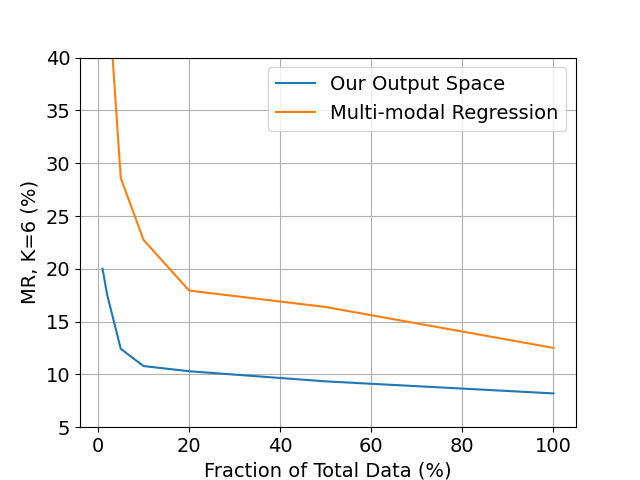
\includegraphics[height=6.6cm]{figures/supp/data_curve.png}
\end{center}
\caption{Model performance when using different amounts of data for training.
  Our output parameterization explicitly leverages lanes as priors for motion
  forecasting, and thus significantly ease the learning compared to directly
  regressing the future motions in the 2D plane.
}
\label{fig:supp_output}
\end{figure}

\begin{table}[t]
  \centering
  \begin{tabular}{ccc|cc}
  \specialrule{.2em}{.1em}{.1em}
  Curve & Velocity & Learnable & $\text{min}_1$ADE & $\text{min}_6$ADE\\
  \hline
  line & const & & 1.53 & 1.04\\
  line & acc & & 1.52 & 1.02\\
  line & acc & \checkmark & 1.41 & 0.86\\
  Bezier & const & & 1.46 & 0.96\\
  Bezier & acc & & 1.44 & 0.94\\
  \rowcolor{grey}Bezier & acc & \checkmark & \textbf{1.33} & \textbf{0.77}\\
  \specialrule{.1em}{.05em}{.05em}

\end{tabular}
\caption{Ablation studies on output parameterizations. We compare different ways
of proposing curves (straight line v.s. Bezier quadratic curve), unrolling
velocities (const as constant velocity and acc as constant acceleration), as well
as using learnable refinement header or not. Our final model is shaded in
\colorbox{grey}{grey}.}
\label{table:supp_refinement}
\end{table}



\begin{figure*}[t]
\centering
\setlength{\tabcolsep}{1pt}
\begin{tabular}{cccc}
  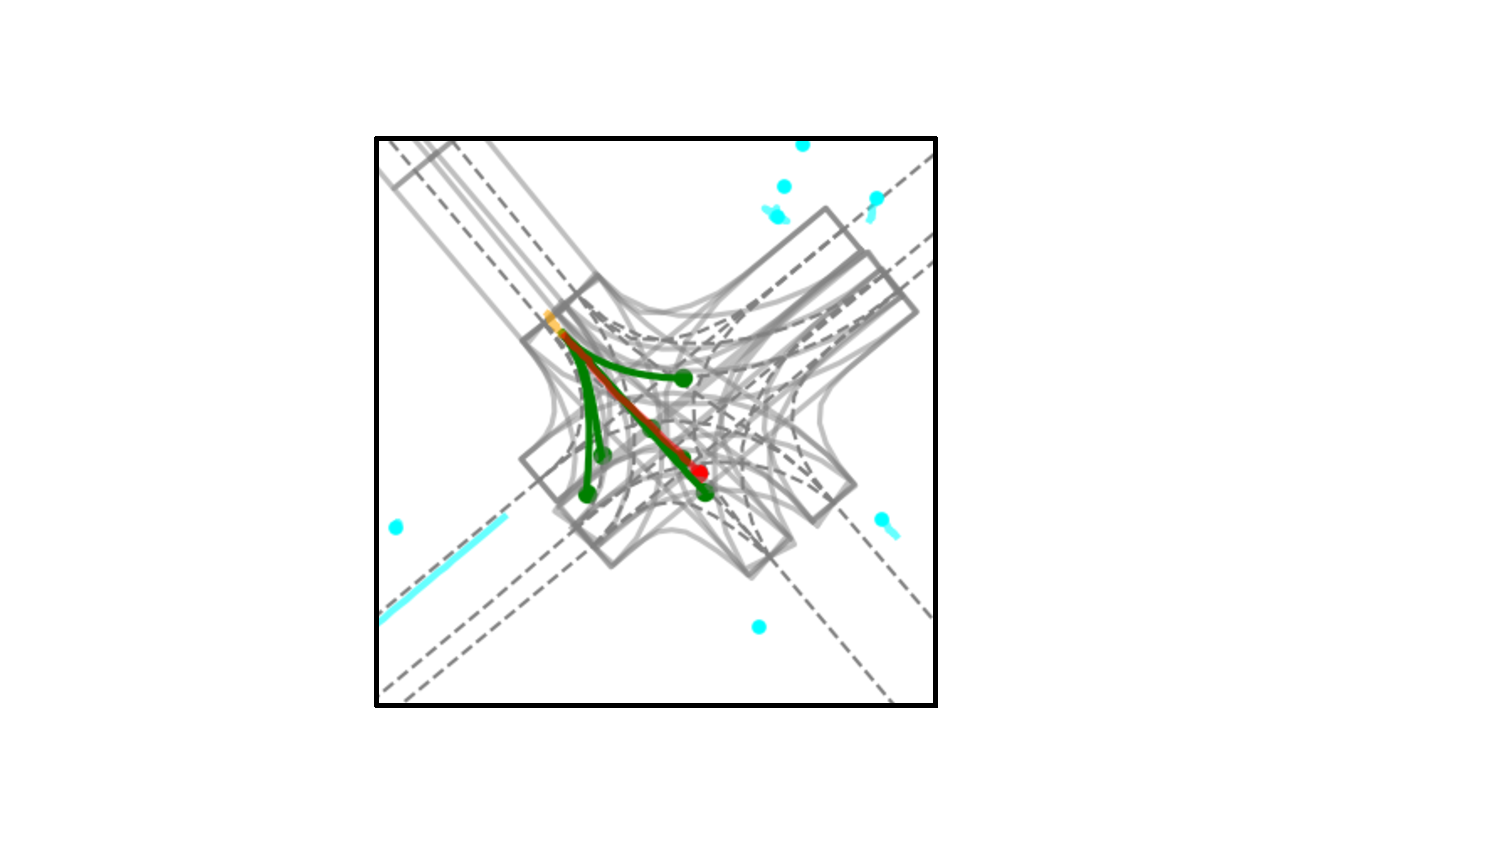
\includegraphics[width=0.24\linewidth]{figures/supp/turning1.pdf}
&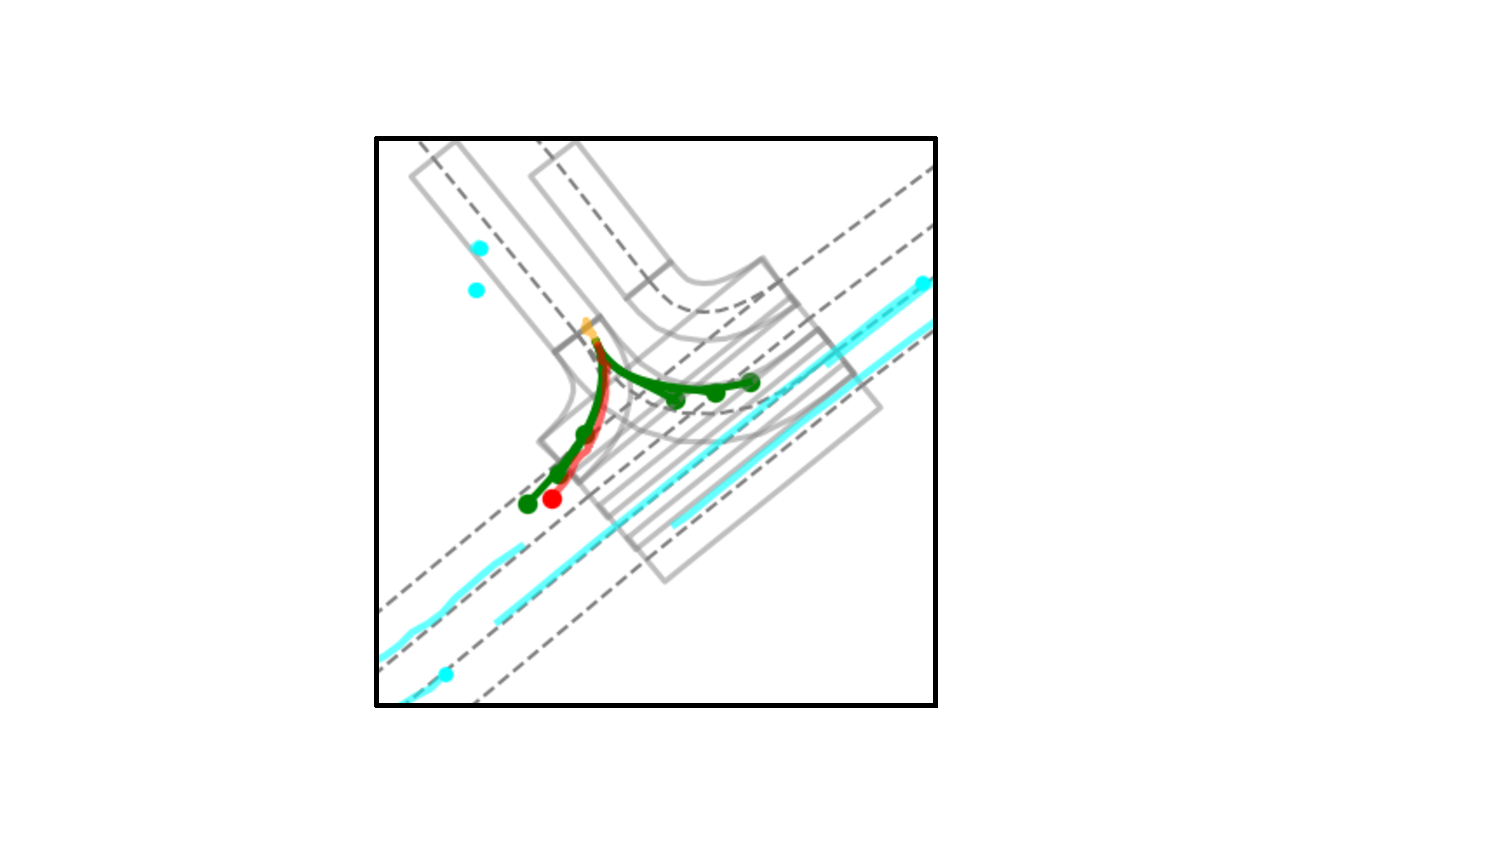
\includegraphics[width=0.24\linewidth]{figures/supp/turning2.pdf}
&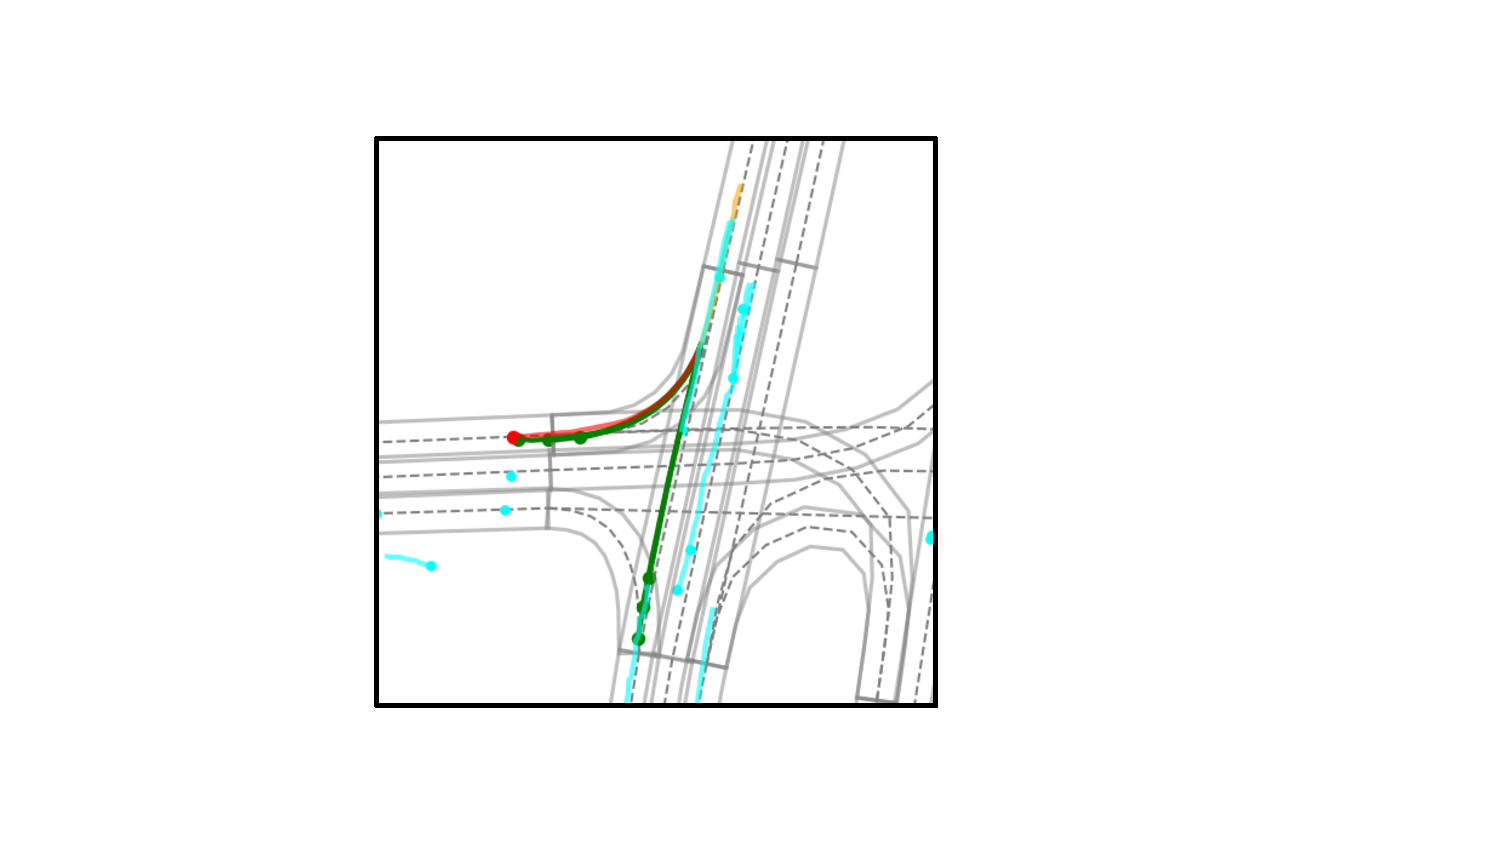
\includegraphics[width=0.24\linewidth]{figures/supp/turning3.pdf}
&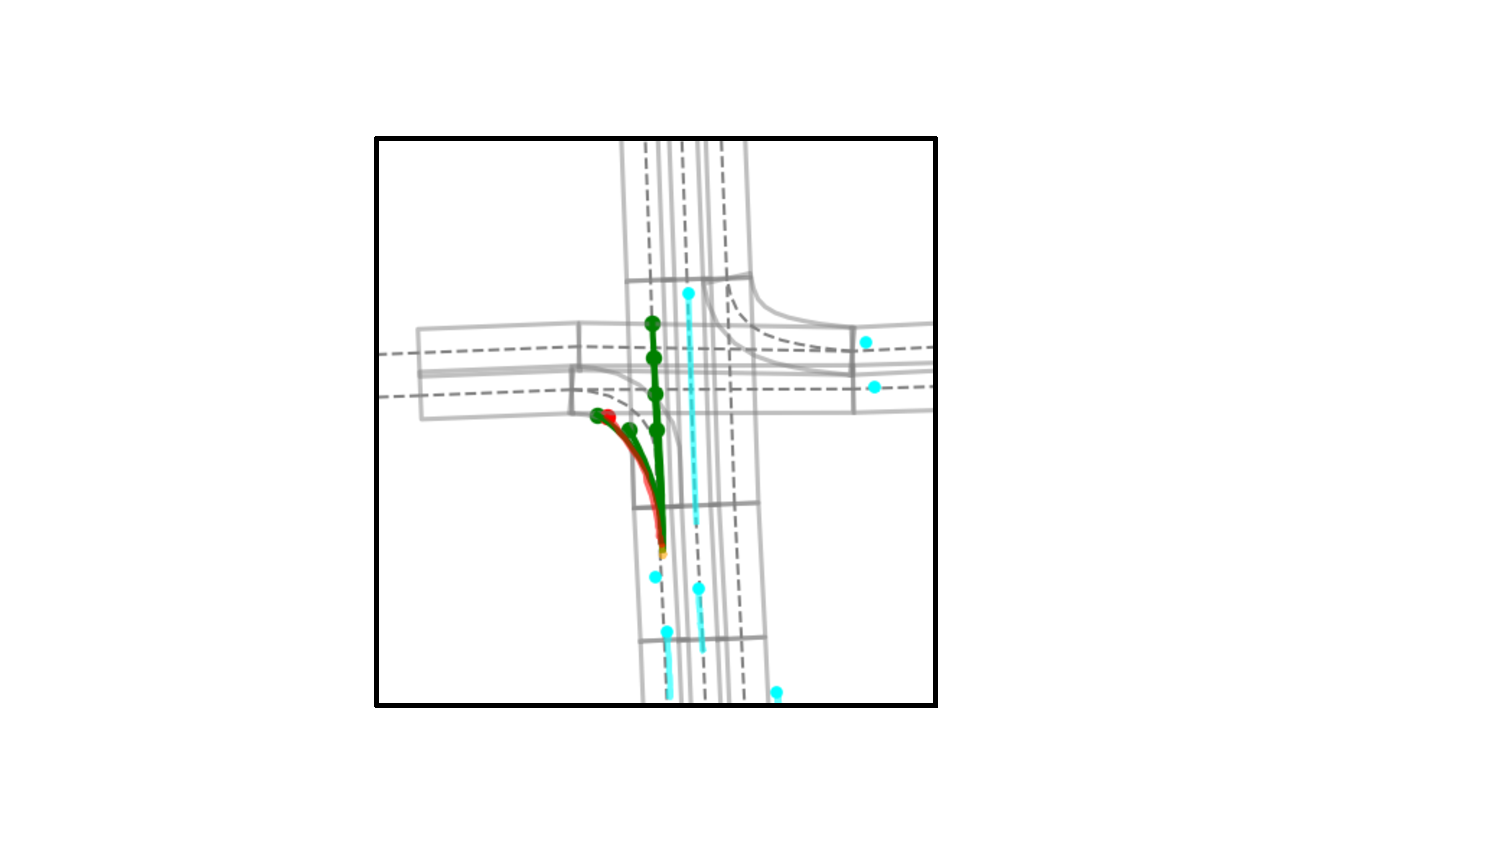
\includegraphics[width=0.24\linewidth]{figures/supp/turning4.pdf}\\
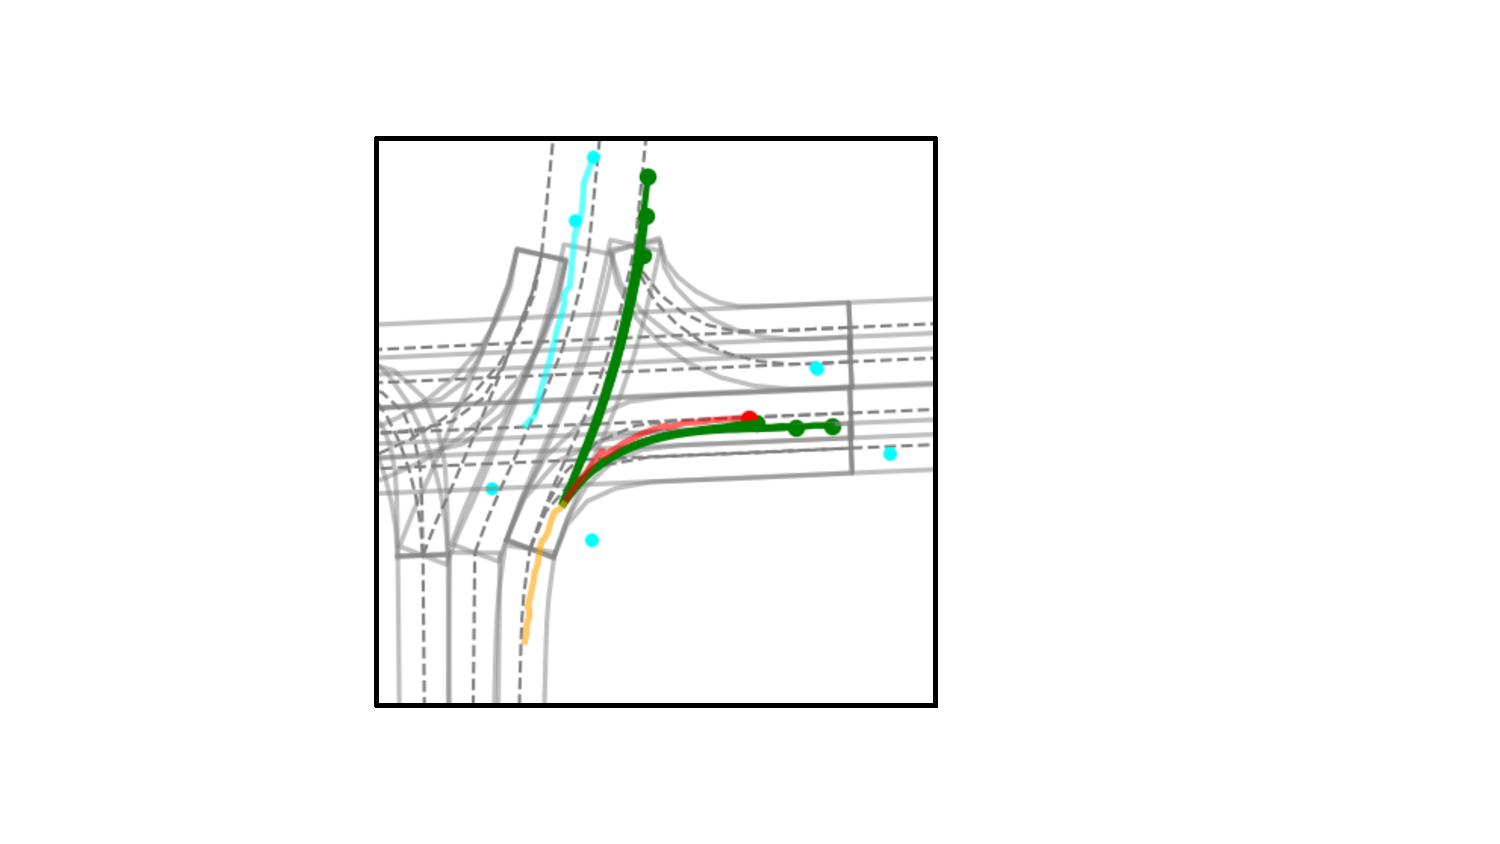
\includegraphics[width=0.24\linewidth]{figures/supp/turning5.pdf}
&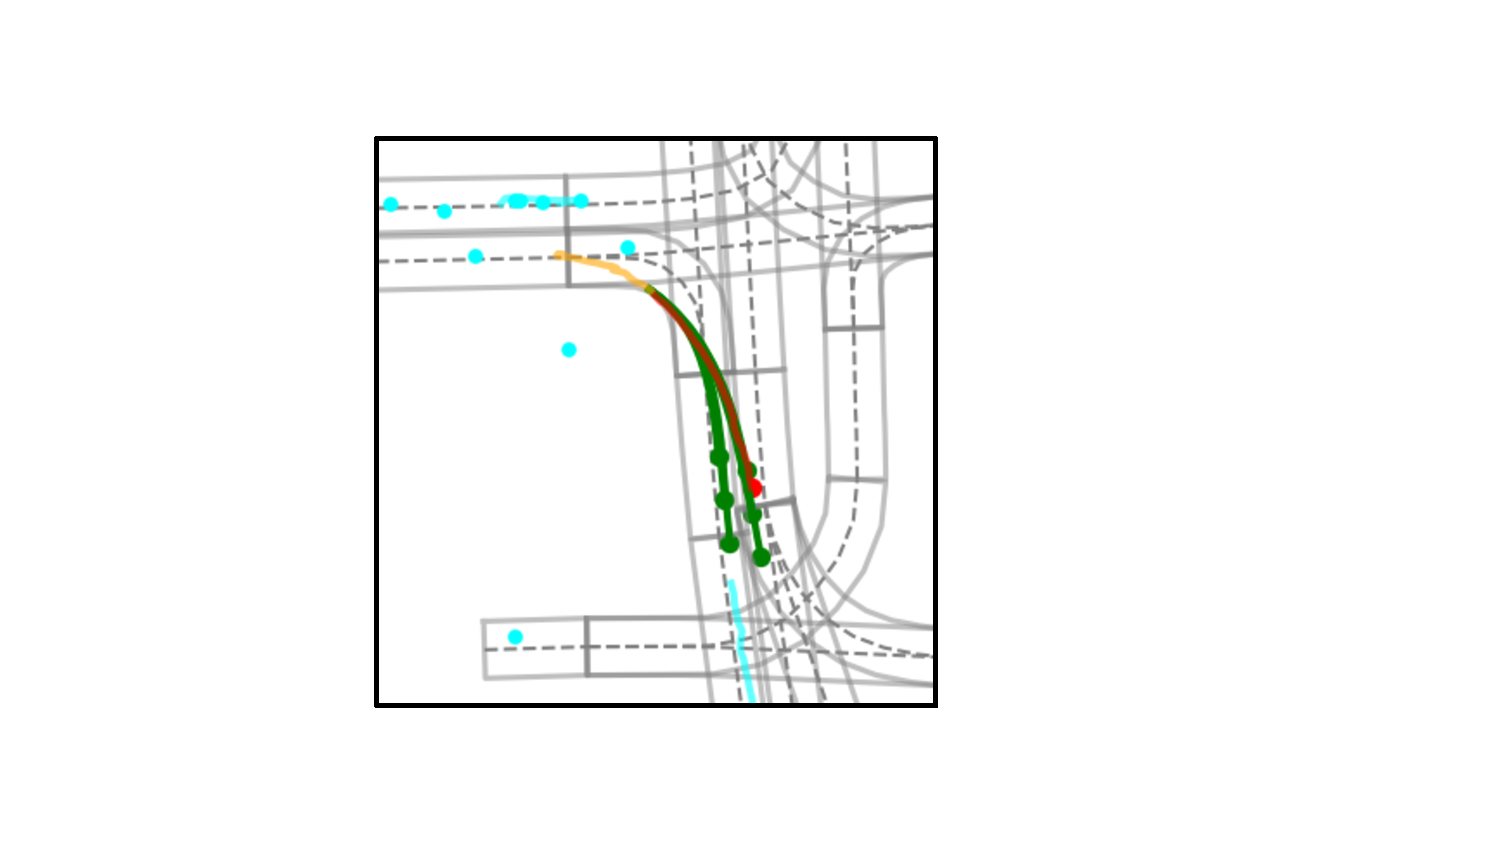
\includegraphics[width=0.24\linewidth]{figures/supp/turning6.pdf}
&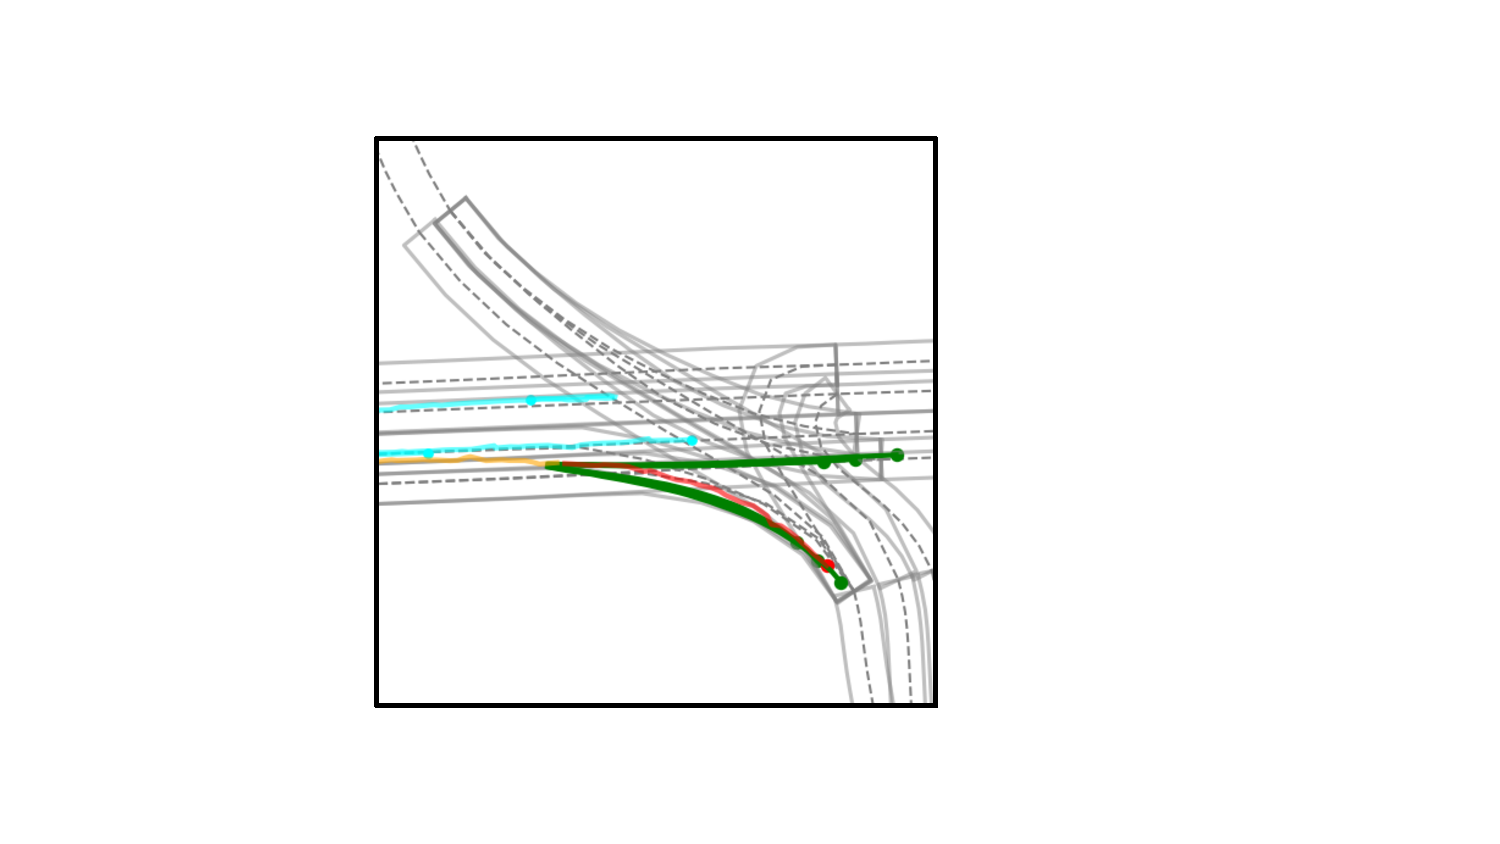
\includegraphics[width=0.24\linewidth]{figures/supp/turning7.pdf}
&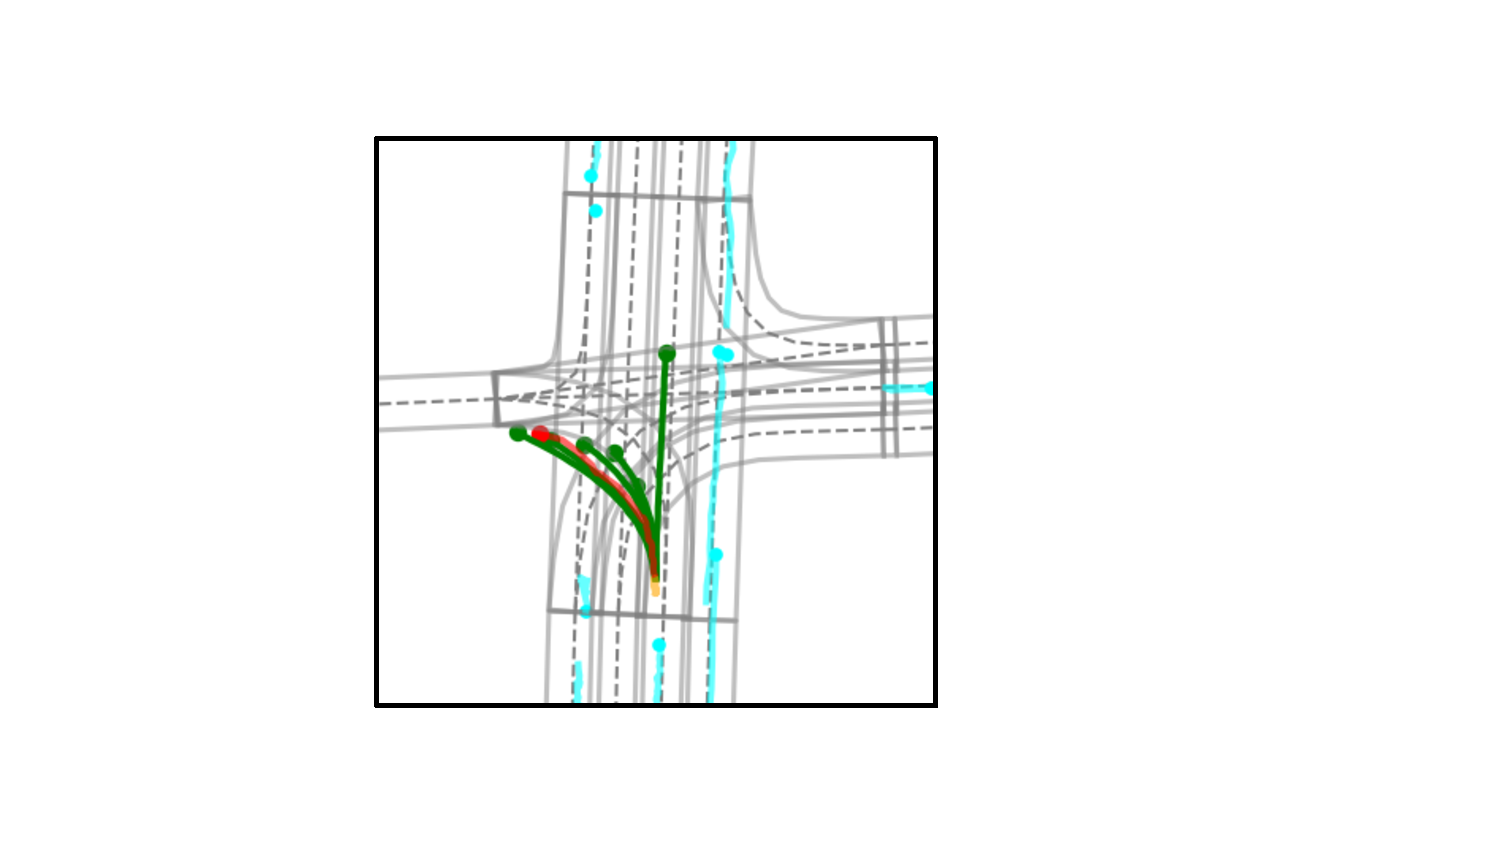
\includegraphics[width=0.24\linewidth]{figures/supp/turning8.pdf}\\
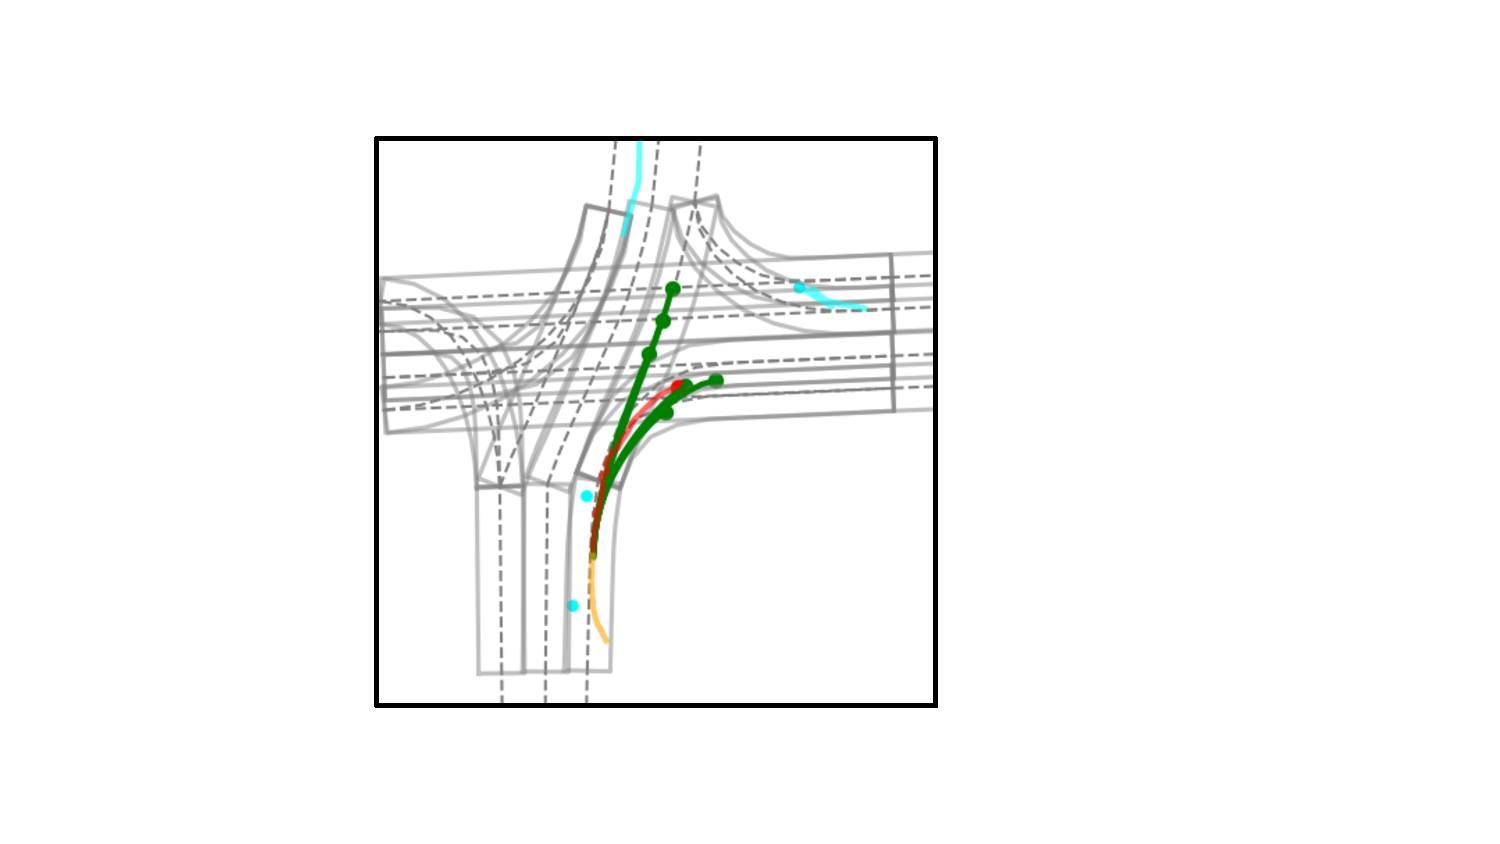
\includegraphics[width=0.24\linewidth]{figures/supp/curve1.pdf}
&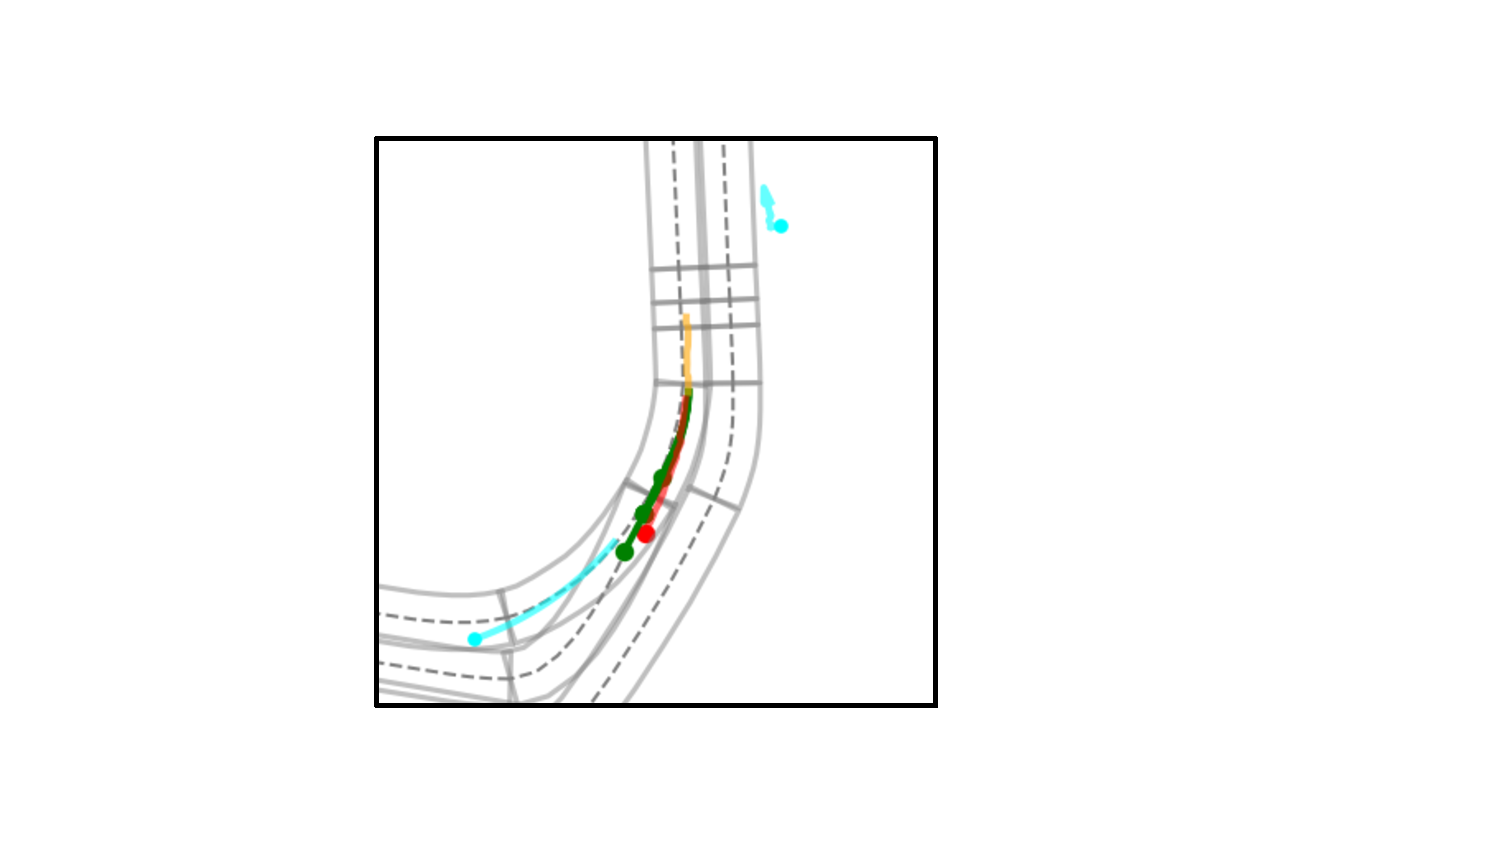
\includegraphics[width=0.24\linewidth]{figures/supp/curve2.pdf}
&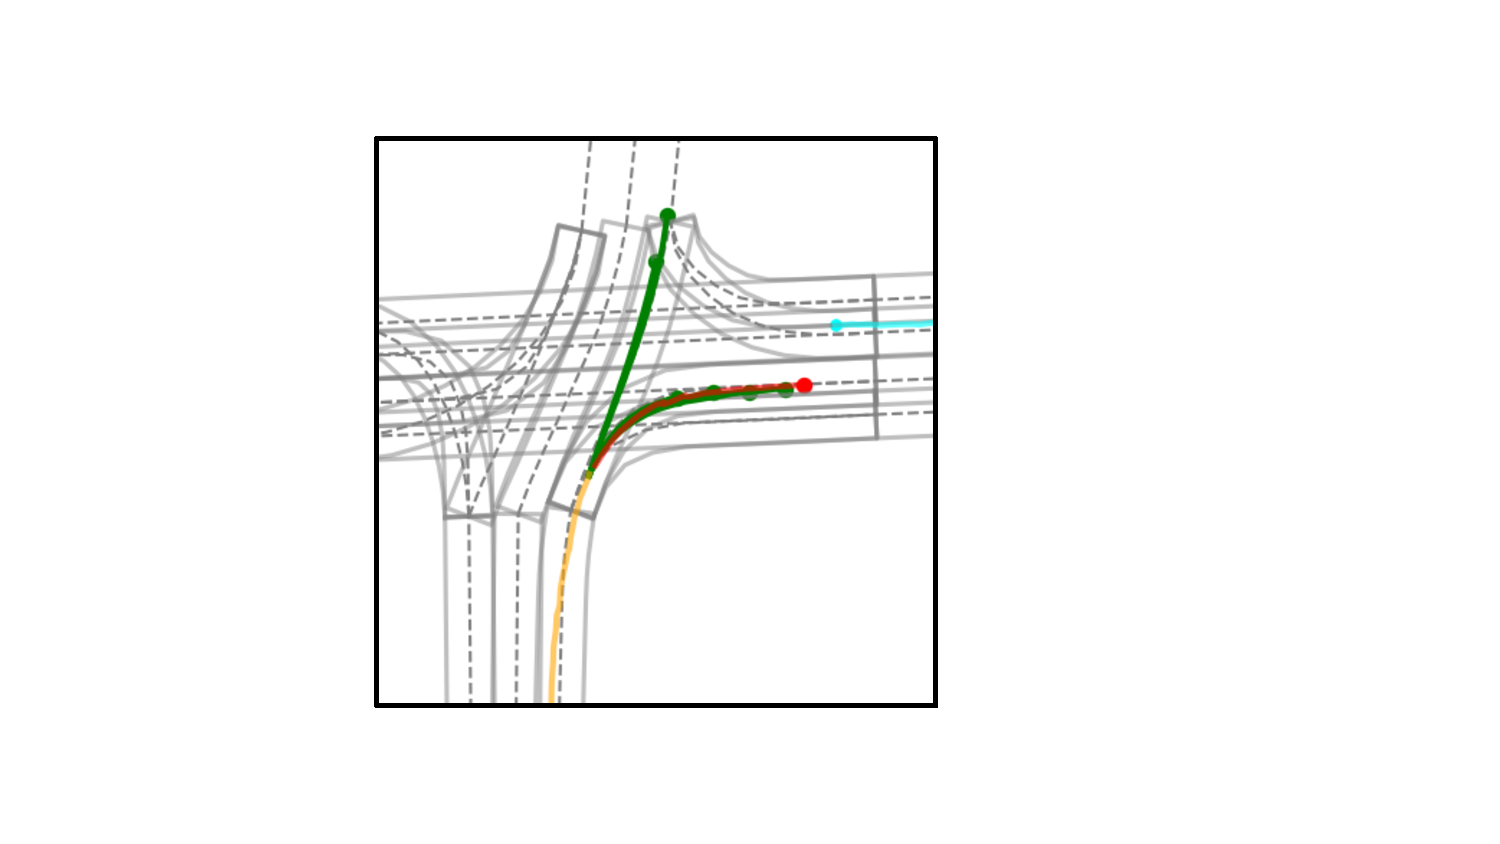
\includegraphics[width=0.24\linewidth]{figures/supp/curve3.pdf}
&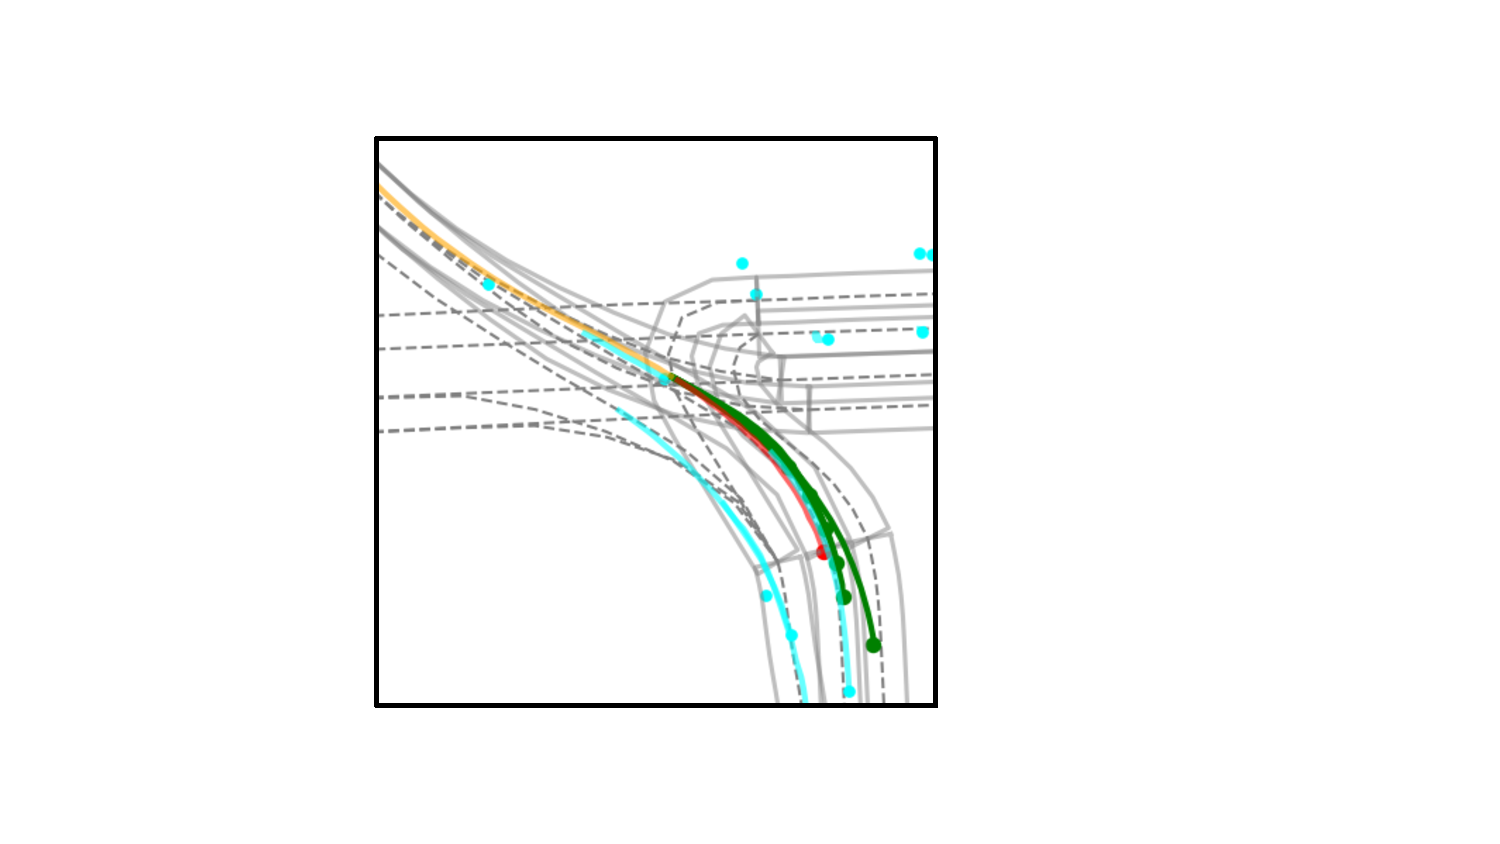
\includegraphics[width=0.24\linewidth]{figures/supp/curve4.pdf}\\
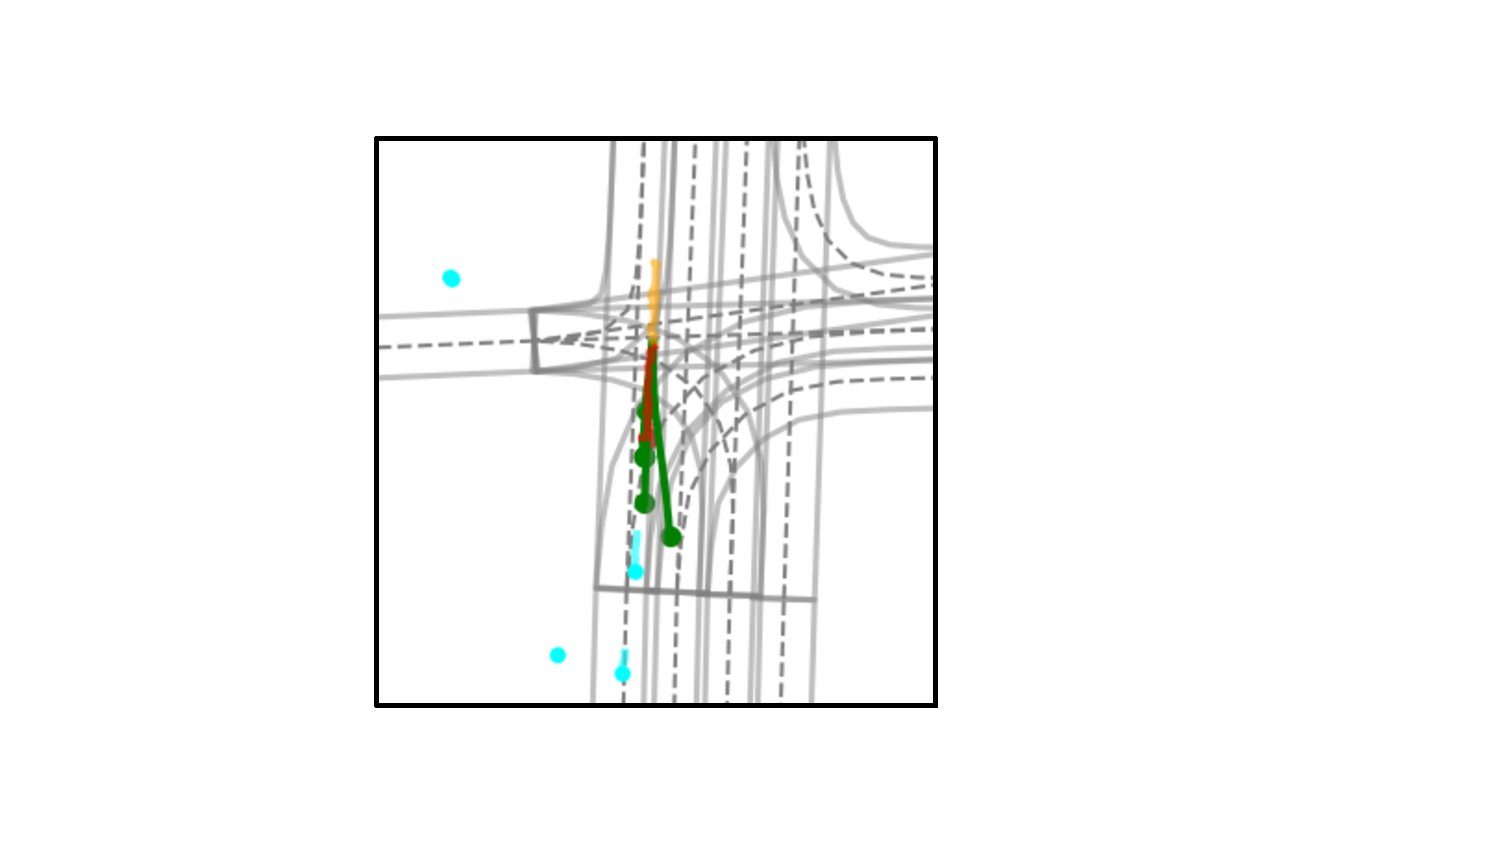
\includegraphics[width=0.24\linewidth]{figures/supp/inter1.pdf}
&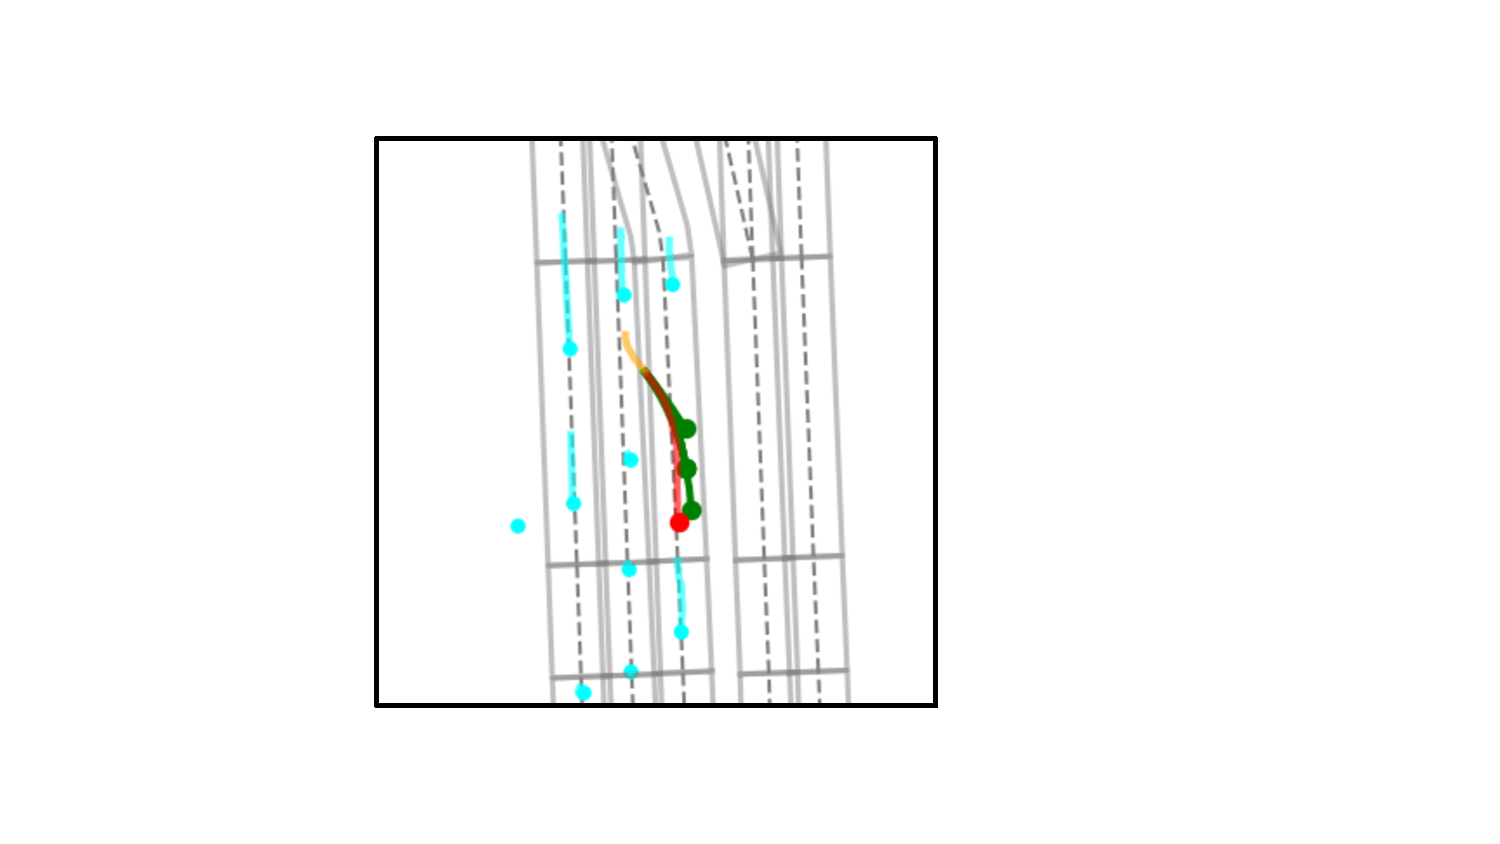
\includegraphics[width=0.24\linewidth]{figures/supp/inter2.pdf}
&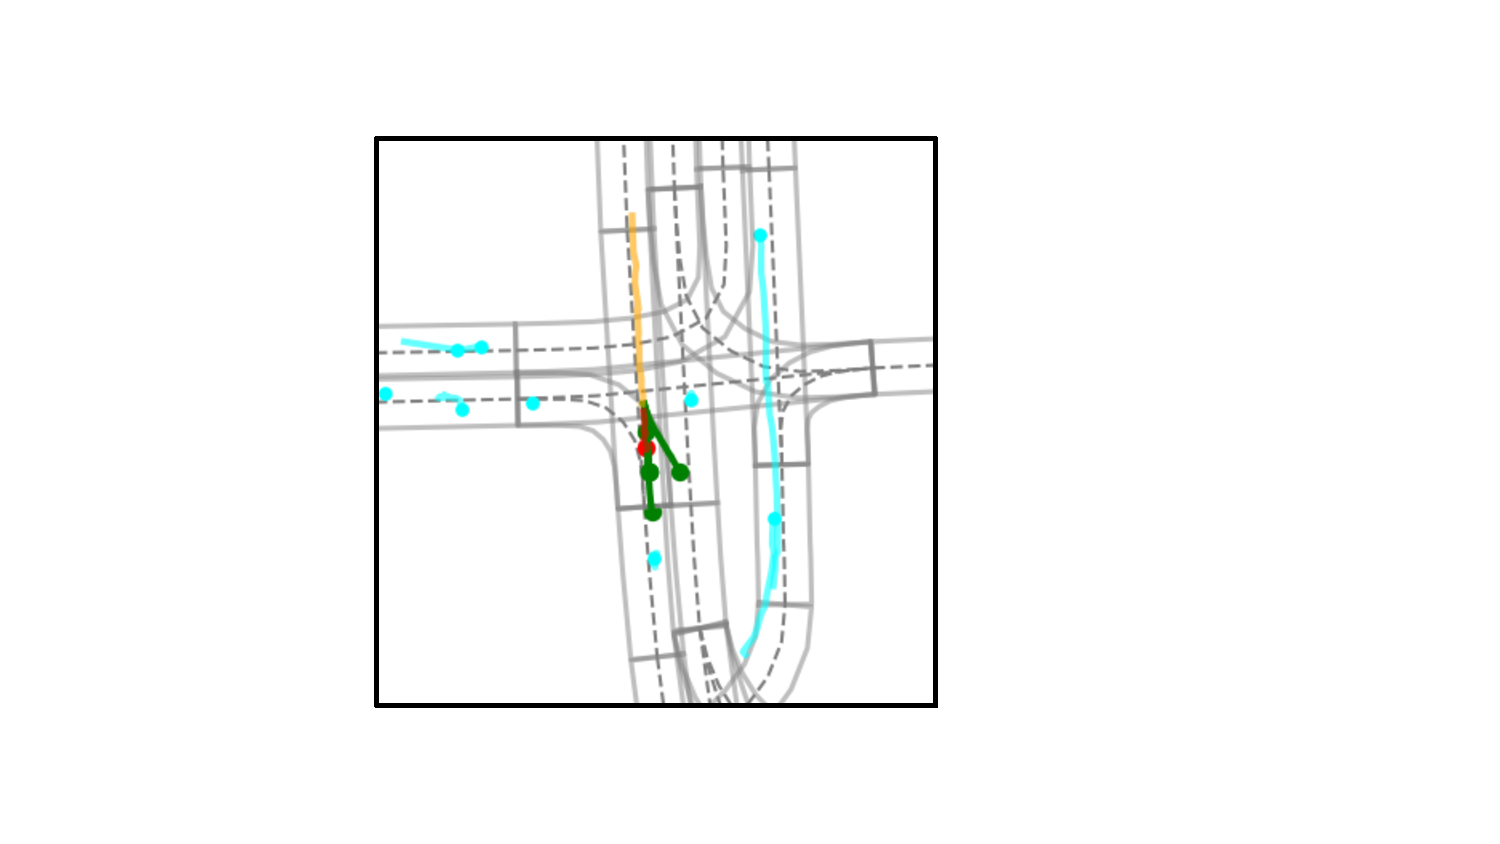
\includegraphics[width=0.24\linewidth]{figures/supp/inter3.pdf}
&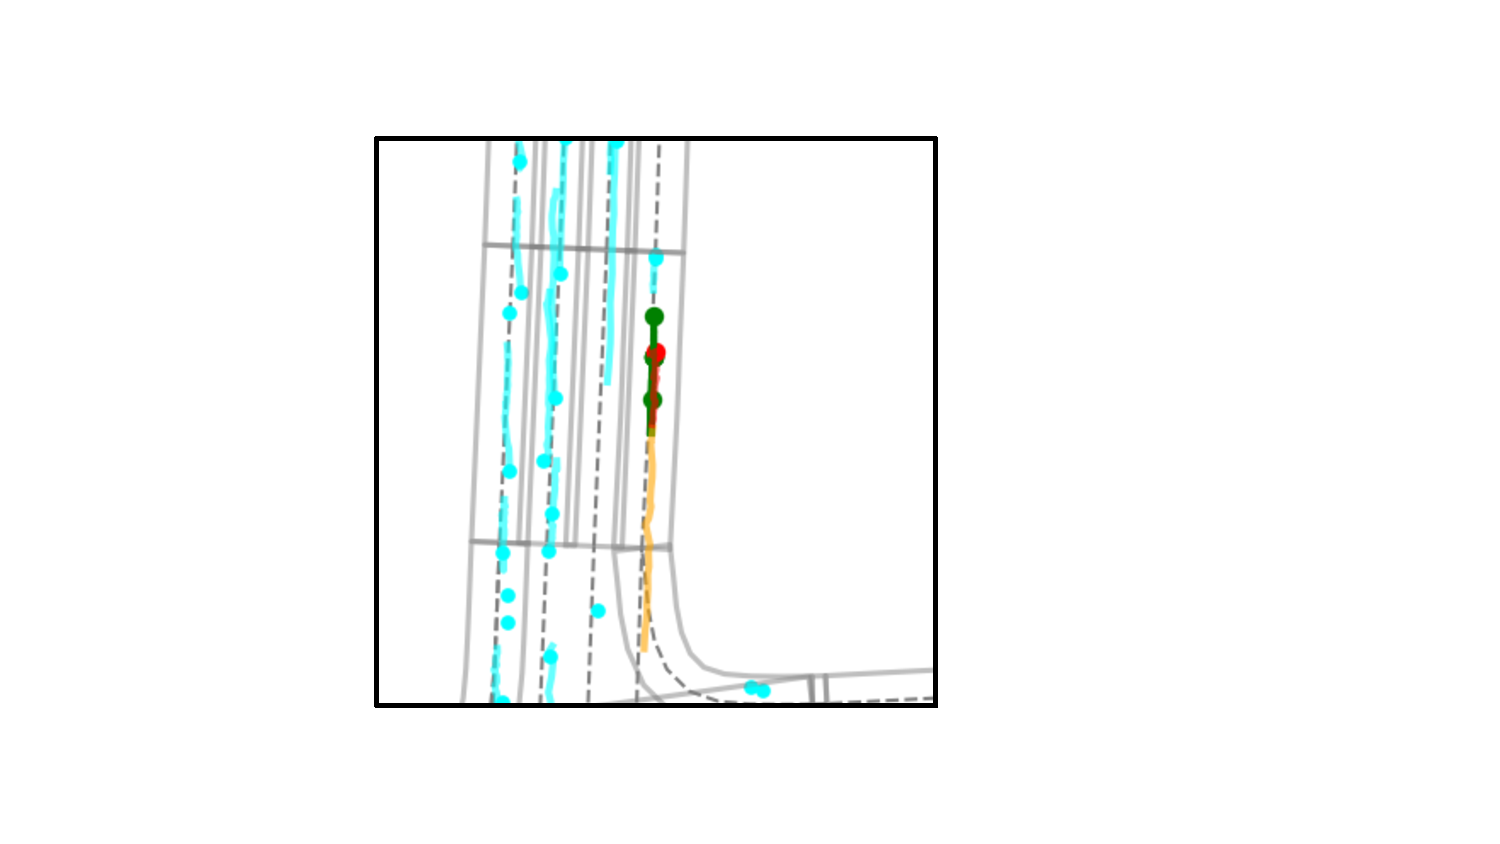
\includegraphics[width=0.24\linewidth]{figures/supp/inter4.pdf}\\
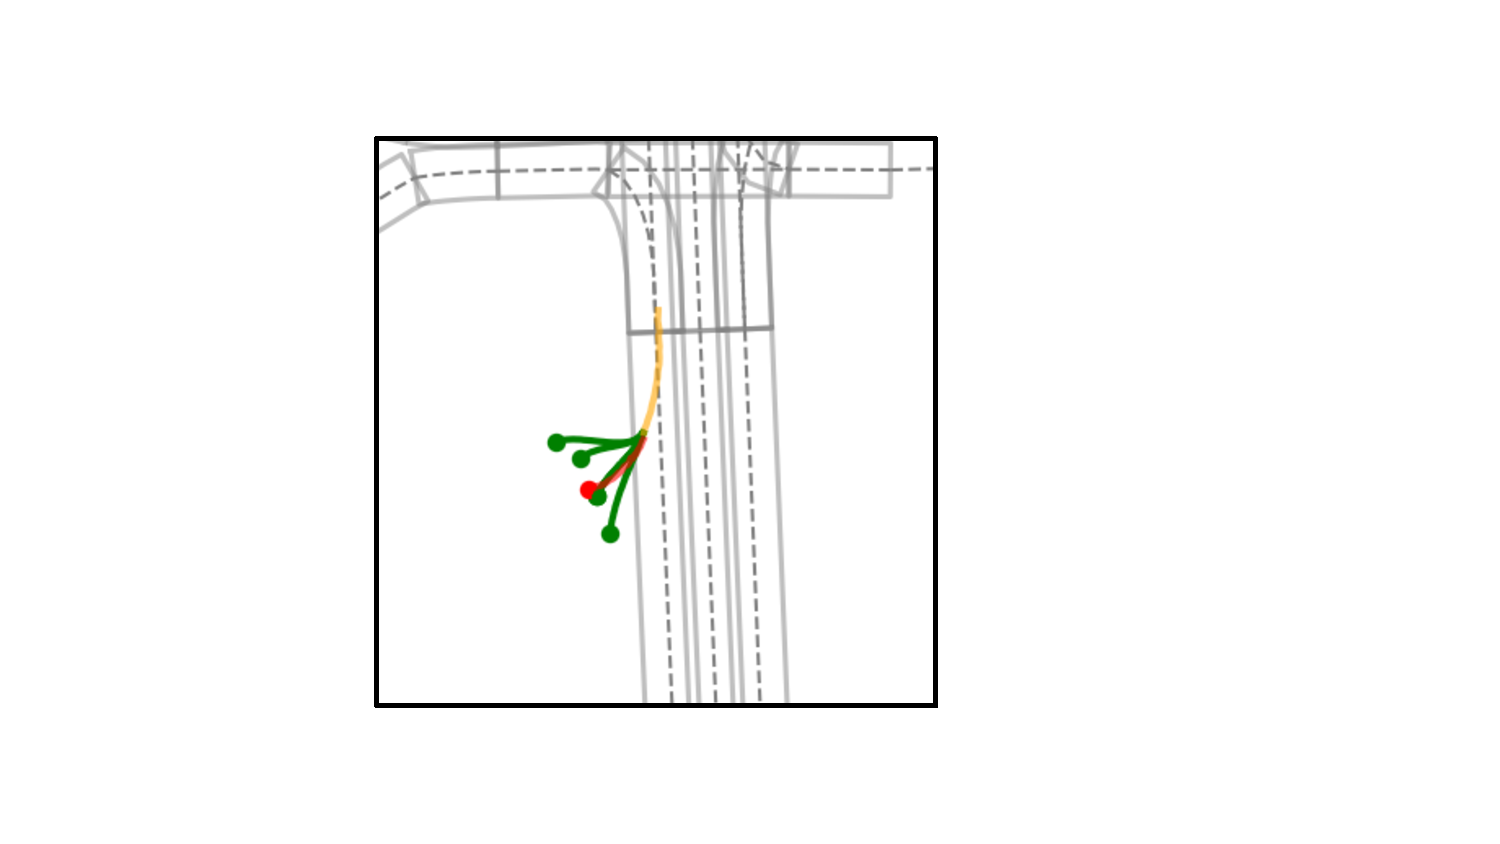
\includegraphics[width=0.24\linewidth]{figures/supp/map1.pdf}
&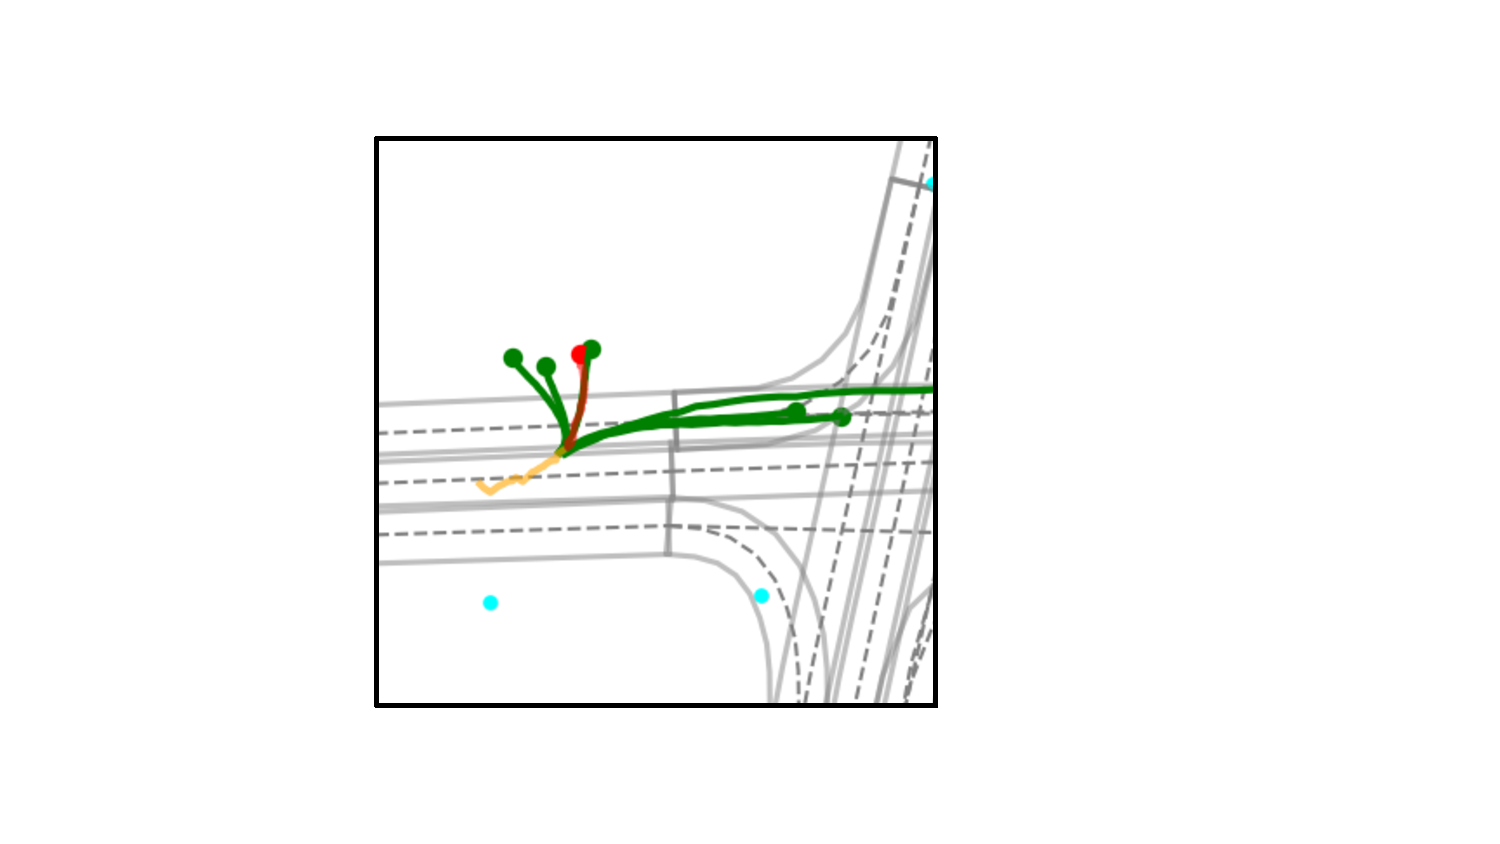
\includegraphics[width=0.24\linewidth]{figures/supp/map2.pdf}
&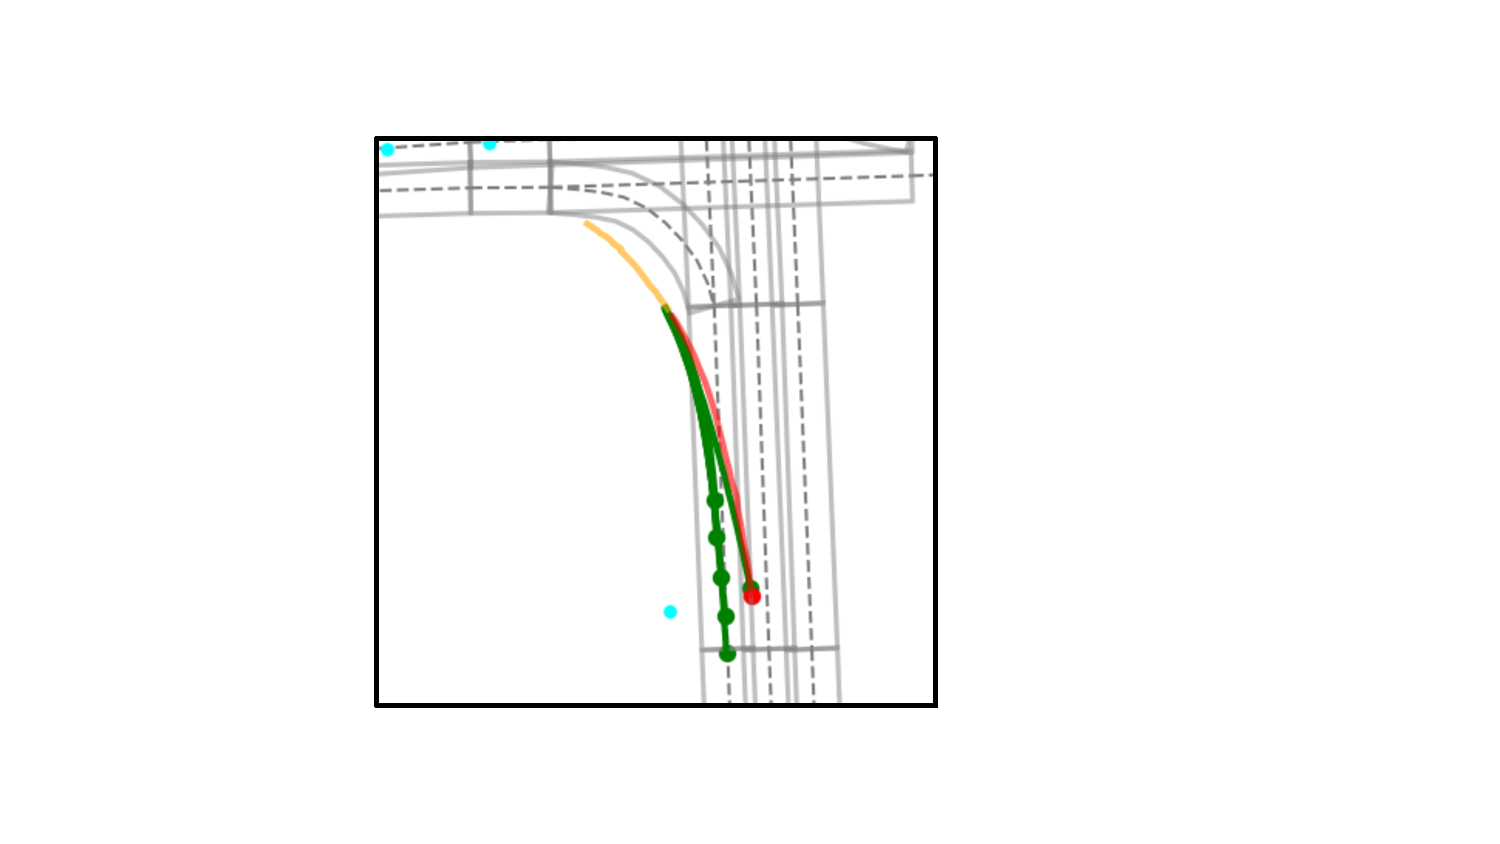
\includegraphics[width=0.24\linewidth]{figures/supp/map3.pdf}
&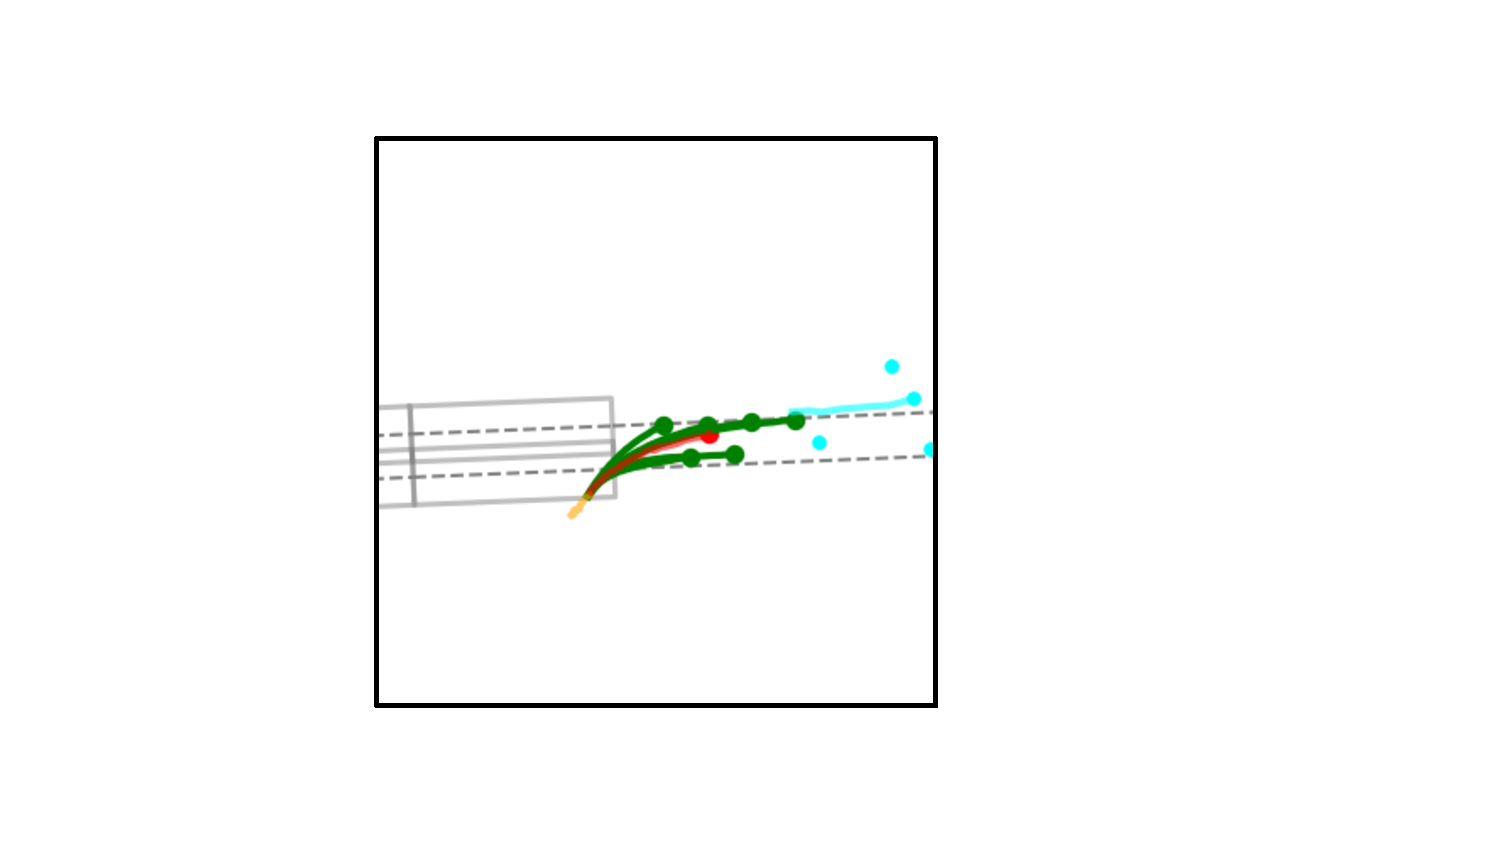
\includegraphics[width=0.24\linewidth]{figures/supp/map4.pdf}\\

\end{tabular}
\caption{Qualitative results on Argoverse validation set. We show a various of
scenarios including, turning (row 1-2), curved roads (row 3), breaking and
overtaking (row 4), abnormal behaviors (row 5).}
\label{fig:supp_vis}
\end{figure*}


\section{Qualitative Results}
\label{sec:supp_qual}
Lastly, we provide more visualization of our model outputs, as we believe the
metric numbers can only reveal part of the story. We present various
scenarios in Fig.~\ref{fig:supp_vis}, including turning, following curved roads,
interacting with other actors and some abnormal behaviors. On the first two
rows, we show turning behaviors under various map topologies. We can see
our motion forecasting results nicely capture possible modes: turning into
different directions or occupying different lanes after turning. We also do well 
even if the actor is not strictly following the centerlines. On the
third row, we show predictions following curved roads, which are difficult
scenarios for auto-regressive predictors \cite{nmp,intentnet}. On the fourth
row, we show that our model can predict breaking or overtaking behaviors when
leading vehicles are blocking the ego-actor. Finally, we show in the fifth row
that our model also works well when abnormal situations occur, \eg, driving out of
roads. This is impressive as the model relies on
lanes to make predictions, yet it shows capabilities to predict non-map-compliant
behaviors.
